Random Early Detection or RED is the algorithm introduced in
\cite{FloydJacobsonRED}. RED monitors the average queue size and when it
exceeds a preset threshold, the router drops the arriving packet with a
certain probability, where the exact probability is a function of the average
queue size. If ECN is active, the packets are choose randomly and marked. When
a connection uses a larger share of available bandwidth, it is more likely to
be marked. The idle periods (periods when the queue is empty) are also take
into account for the calculations of the average queue size.

The objectives behind the  implementation of RED are:
\begin{enumerate}
\item Minimize packet loss and queue delay.
\item Avoid global synchronization of sources by randomize its marking
decision and by spacing out its marking.
\item Maintain high link utilization.
\item remove biases against bursty sources by limiting the queue occupancy so
that there is always room left in the queue to buffer transient.
\end{enumerate}

\begin{wrapfigure}{r}{0.5\textwidth}
  \begin{center}
    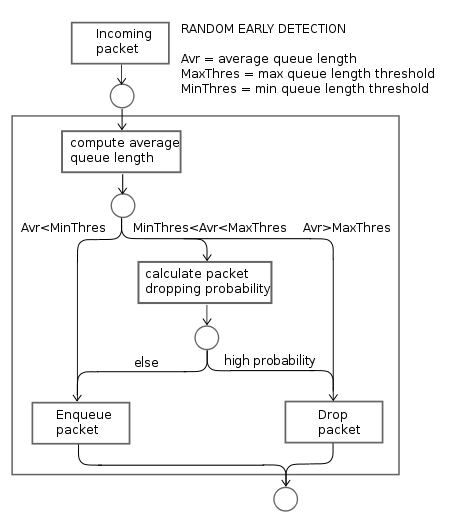
\includegraphics[width=0.48\textwidth]{img/RED}
  \end{center}
  \caption{RED's Flowchart}
  \label{fig:RED}
\end{wrapfigure}

Because RED can control the average queue size while accommodating transient
congestion, implementing RED in routers can provide high throughput and low
average delay in high-speed networks with TCP connections that have large
windows. Also, in routers where RED and ECN are implemented the bursty traffic
is well handled and the global synchronization between flows is avoided by
decreasing their window at the same time.

The most common critics to RED is its complexity to properly configure its
parameters. It is because of this that after their official publication, it
was necessary to perform the second publication \cite{NotesRED}, which aims to
explain a few more details on how to configure it properly. Since RED rely on
queue length as index of congestion, it can reflect the presence of congestion
but not the severity nor the numbers of competing connections sharing the
link. Since long ago networks ceased have a static configuration, RED require
a wide range of parameters to operate correctly under different congestion
scenarios. Unfortunately, this failure leads to deterministically mark packets
and suffer from poor link utilization. \textit{While  ECN timeouts allows RED
to avoid packet loss, the deterministic marking eventually causes
underutilization at the bottleneck link}\cite{FengBLUEAQM}.

As stated in \cite{NicholsJacobsonCQD}, \textit{RED was simple and can be
effective at reducing persistent queues, little guidance was available to set
its configuration parameters and it functioned poorly in a number of cases.
This led to a general reluctance to use it}.

Also to archive the ideal operating point, it can only do so when it has a
sufficient amount of buffer space, which leads to default induce an extra
latency.
